\paragraph{QuizziPedia::Front-End::ModelViews::QuestionsModelView}

\label{QuizziPedia::Front-End::ModelViews::QuestionsModelView}

\begin{figure}[ht]
	\centering
	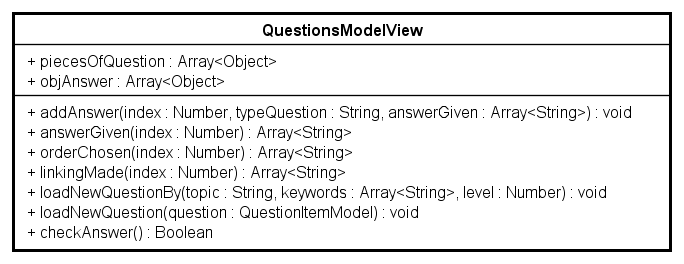
\includegraphics[scale=0.75,keepaspectratio]{UML/Classi/Front-End/QuizziPedia_Front-end_ModelView_QuestionsModelView.png}
	\caption{QuizziPedia::Front-End::ModelViews::QuestionsModelView}
\end{figure} \FloatBarrier

\begin{itemize}
	\item \textbf{Descrizione}: classe di tipo modelview la cui istanziazione è contenuta all'interno della variabile di ambiente \texttt{\$scope} di \textit{Angular\ped{G}}. All'interno di essa sono presenti le variabili e i metodi necessari per il \textit{Two-Way Data-Binding\ped{G}} tra le \textit{directives\ped{G}} che compongono dinamicamente la vista della domanda e il \textit{controller\ped{G}} \texttt{QuestionsController};
	\item \textbf{Utilizzo}: viene utilizzata per effettuare il \textit{Two-Way Data-Binding\ped{G}} tra le \textit{directives\ped{G}} che compongono dinamicamente la vista della domanda e il \textit{controller\ped{G}} \texttt{QuestionsController} rendendo disponibili variabili e metodi;
	\item \textbf{Relazioni con altre classi}: 
	\begin{itemize} 
		\item \textbf{OUT \texttt{QuestionsController}}: questa classe permette di gestire il recupero delle domande per poterle stampare nella modalità allenamento;
		\item \textbf{OUT \texttt{ClickableAnswerDirective}}: rappresenta il componente grafico che permette all'utente di visualizzare la domanda ad area cliccabile nell'immagine. Viene visualizzato dinamicamente all'interno delle \textit{views\ped{G}} \texttt{TrainingView} e \texttt{FillingQuestionnaireView} mediante il \textit{controller\ped{G}} \texttt{QuestionsController};
		\item \textbf{OUT \texttt{EmptySpaceAnswerDirective}}: rappresenta il componente grafico che permette all'utente di visualizzare l'esercizio a riempimento di spazi vuoti. Viene visualizzato dinamicamente all'interno delle \textit{views\ped{G}} \texttt{TrainingView} e \texttt{FillingQuestionnaireView} mediante il \textit{controller\ped{G}} \texttt{QuestionsController};
		\item \textbf{OUT \texttt{HeaderTextQuestionDirective}}: rappresenta il componente grafico che presenta all'utente l'argomento, le parole chiave e il numero di domande complessive. Viene visualizzato dinamicamente all'interno delle \textit{views\ped{G}} \texttt{TrainingView} e \\\texttt{FillingQuestionnaireView} mediante il \textit{controller\ped{G}} \texttt{QuestionsController};
		\item \textbf{OUT \texttt{LinkingAnswerDirective}}: rappresenta il componente grafico che permette all'utente di visualizzare la domanda di collegamento. Viene visualizzato dinamicamente all'interno delle \textit{views\ped{G}} \texttt{TrainingView} e \texttt{FillingQuestionnaireView} mediante il \textit{controller\ped{G}} \texttt{QuestionsController};
		\item \textbf{OUT \texttt{MultipleChoiceAnswerDirective}}: rappresenta il componente grafico che permette all'utente di visualizzare la domanda a risposta multipla. Viene visualizzato dinamicamente all'interno delle \textit{views\ped{G}} \texttt{TrainingView} e \texttt{FillingQuestionnaireView} mediante il \textit{controller\ped{G}} \texttt{QuestionsController};
		\item \textbf{OUT \texttt{SortImagesAnswerDirective}}: rappresenta il componente grafico che permette all'utente di visualizzare la domanda ad ordinamento di immagini. Viene visualizzato dinamicamente all'interno delle \textit{views\ped{G}} \texttt{TrainingView} e \texttt{FillingQuestionnaireView} mediante il \textit{controller\ped{G}} \texttt{QuestionsController};
		\item \textbf{OUT \texttt{SortTextAnswerDirective}}: rappresenta il componente grafico che permette all'utente di visualizzare la domanda ad ordinamento di stringhe. Viene visualizzato dinamicamente all'interno delle \textit{views\ped{G}} \texttt{TrainingView} e \texttt{FillingQuestionnaireView} mediante il \textit{controller\ped{G}} \texttt{QuestionsController};
		\item \textbf{OUT \texttt{TrueFalseAnswareDirective}}: rappresenta il componente grafico che permette all'utente di visualizzare la domanda vero e falso. Viene visualizzato dinamicamente all'interno delle \textit{views\ped{G}} \texttt{TrainingView} e \texttt{FillingQuestionnaireView} mediante il \textit{controller\ped{G}} \texttt{QuestionsController};	
		\item \textbf{OUT \texttt{TrainingView}}: \textit{view\ped{G}} principale della modalità allenamento, conterrà i vari templates di ogni domanda dell'allenamento.				
	\end{itemize}
	\item \textbf{Attributi}: 
	\begin{itemize}
		\item \texttt{+ piecesOfQuestion: Array<Object>} \\
		Questo attributo è un \texttt{array} di \texttt{Object} contenente la domanda da visualizzare dinamicamente attraverso le direttive all'interno le direttive di allenamento e di compilazione dei questionari;
		\item \texttt{+ objAnswer: Array<Object>} \\
		Questo attributo è un \texttt{array} di \texttt{Object} contenente le risposte date fino a quel momento dall'utente in una domanda. L'\texttt{Object} è così formato: \\
		\begin{itemize}
			\item \texttt{+ typeQuestion: String} \\
			Questo attributo rappresenta il tipo della domanda;
			\item \texttt{+ answerGiven: Array<String>} \\
			Questo attributo rappresenta le riposte scelte dall'utente fino a quel momento. Può essere creato con una funzione di \textit{callback\ped{G}}.
		\end{itemize}
	\end{itemize}
	\item \textbf{Metodi}: 
	\begin{itemize}
	\item \texttt{+} \texttt{addAnswer(index: Number, typeQuestion: String, answerGiven: \\Array<String>): void} \\
	Metodo che gestisce l'evento di selezione delle risposte. \\
	\textbf{Parametri}:
	\begin{itemize}
		\item \texttt{index: Number} \\
		Parametro contenente l'indice della risposta di cui si vuole tenere traccia. Rappresenta anche l'indice dell'array \texttt{answerGiven} in cui verrà inserito l'oggetto delle risposte date;
		\item \texttt{typeQuestion: String} \\
		Parametro contenente una stringa la quale indica la tipologia della domanda;
		\item \texttt{answerGiven: Array<String>} \\
		Parametro contenente l'array di risposte date dall'utente aggiornato all'ultima iterazione.
	\end{itemize}
	\item \texttt{+} \texttt{save(index: Number): Array<String>} \\
	Metodo di supporto che ritorna un array di stringhe contenente le risposte date. Si occupa di recuperare le risposte date nelle domande vero/falso, risposta multipla e ad area cliccabile.\\
	\textbf{Parametri}:
	\begin{itemize}
		\item \texttt{index: Number} \\
		Parametro contenente l'indice della risposta di cui si vuole raccogliere le risposte date. 
	\end{itemize}
	\item \texttt{-} \texttt{downloadNextQuestionTraining(nextQuestion: Object): void} \\
	Metodo che gestisce l'evento per scaricare una nuova domanda in base ai parametri passati. Evoca l'evento per inserire la domanda in \texttt{TrainingModelView}. \\
	\textbf{Parametri}:
	\begin{itemize}
		\item \texttt{nextQuestion: Object} \\
		Parametro contenente un oggetto così fatto: \\
		\textbf{Parametri}:
		\begin{itemize}
			\item \texttt{language: String} \\
			Parametro contenente la lingua della domanda;
			\item \texttt{topic: String} \\
			Parametro contenente l'argomento della domanda;
			\item \texttt{keywords: Array<String>} \\
			Parametro contenente un array di stringhe che rappresenta le keywords scelte per l'allenamento;
			\item \texttt{level: Number} \\
			Parametro contenente il livello dell'utente;
			\item \texttt{alreadyAnswered: Array<String>} \\
			Parametro contenente un array di stringhe che rappresenta le domande già risposte fino a quel momento dell'allenamento;
		\end{itemize}
	\end{itemize}
	\item \texttt{-} \texttt{loadNextQuestionQuiz(question: QuestionItemModel): void} \\
	Metodo che gestisce l'evento per visualizzare una nuova domanda. \\
	\textbf{Parametri}:
	\begin{itemize}
		\item \texttt{question: QuestionItemModel} \\
		Parametro contenente un riferimento all'oggetto di tipo \texttt{QuestionItemModel}.
	\end{itemize}
	\item \texttt{+} \texttt{checkAnswer(): Boolean} \\ 
	Metodo che controlla che le risposte date siano corrette;
	\item \texttt{+} \texttt{dragnNDropQuestions(event: Object, ui: Object, index: Number, type: String, obj: Array<String>): void} 
	Metodo che gestisce l'evento per l'inserimento delle risposte date con una domanda che ha il trascinamento come base di interazione con l'utente. \\
	\textbf{Parametri}:
	\begin{itemize}
		\item \texttt{(event: Object} \\
		Parametro necessario per catturare l'evento di trascinamento;
		\item \texttt{ui: Object} \\
		Parametro necessario per capire quale oggetto viene trascinato;
		\item \texttt{index: Number} \\
		Parametro contenente l'indice della risposta di cui si vuole tenere traccia. Rappresenta anche l'indice dell'array \texttt{answerGiven} in cui verrà inserito l'oggetto delle risposte date;
		\item \texttt{typeQuestion: String} \\
		Parametro contenente una stringa la quale indica la tipologia della domanda;
		\item \texttt{answerGiven: Array<String>} \\
		Parametro contenente l'array di risposte date dall'utente aggiornato all'ultima iterazione.
	\end{itemize}
	\item \texttt{-} \texttt{\$on('loadNewQuestion': String, callback: function): void} \\
	Metodo che gestisce l'evento per scaricare una nuova domanda. \\
	\textbf{Parametri}:
	\begin{itemize}
		\item \texttt{-} \texttt{'loadNewQuestion': String: String} \\
		Parametro che indica su quale evento rimanere in ascolto;
		\item \texttt{-} \texttt{callback: function} \\
		Parametro che indica una funzione da eseguire.
	\end{itemize}
	\item \texttt{+} \texttt{\$on('loadNewQuestionQuiz': String, callback: function): void} \\
	Metodo che gestisce l'evento per caricare una nuova domanda di un questionario.\\
	\textbf{Parametri}:
	\begin{itemize}
		\item \texttt{-} \texttt{'loadNewQuestionQuiz': String} \\
		Parametro che indica su quale evento rimanere in ascolto;
		\item \texttt{-} \texttt{callback: function} \\
		Parametro che indica una funzione da eseguire.
	\end{itemize}
	\item \texttt{+} \texttt{\$on('checkAnswerEvent': String, callback: function): void} \\
	Metodo che gestisce l'evento per lanciare la catena di operazioni per la correzione di una domanda. \\
	\textbf{Parametri}:
	\begin{itemize}
		\item \texttt{-} \texttt{'checkAnswerEvent': String} \\
		Parametro che indica su quale evento rimanere in ascolto;
		\item \texttt{-} \texttt{callback: function} \\
		Parametro che indica una funzione da eseguire.
	\end{itemize}
	\end{itemize}
\end{itemize}

	